\section{Introduction}

Decoherence due to the interaction of a quantum system with its environment presents a significant challenge to scalable quantum computation \cite{nielsen_chuang_2010}.
The requirement that one be able to control and measure the information stored in the quantum system prevents its complete isolation from the environment: for instance, a superconducting transmon qubit must be coupled to microwave readout and control lines, which necessarily increases the uncontrolled interaction of the qubit with its environment \cite{devoret_2013,wendin_2017}.
For large-scale quantum computation to become feasible, methods of preventing, detecting, and correcting errors due to decoherence must be developed.

Typical quantum error correction (QEC) schemes involve redundantly distributing quantum information over multiple physical qubits to form a single logical qubit \cite{nielsen_chuang_2010,wendin_2017,devoret_2013,raussendorf_2012}.
For example, multiple superconducting qubits may be coupled to one another such that the information constituting a single logical qubit is distributed over the entire entangled system.
Because the environmental noise which causes decoherence is generally only locally correlated, quantum information stored non-locally is protected.

The system used to encode a logical qubit, however, need not be composed of multiple two-level systems.
The non-local phase space of a single oscillator may instead be used to encode quantum information; such encodings are called bosonic codes \cite{cai_2021}.
A logical qubit is encoded as a superposition of (potentially infinitely many) resonator Fock states.
These encodings are advantageous due to the fact that they utilize only a single resonator, and therefore require far fewer physical resources per qubit than other QEC schemes.

\begin{figure}[t]
    \centering
    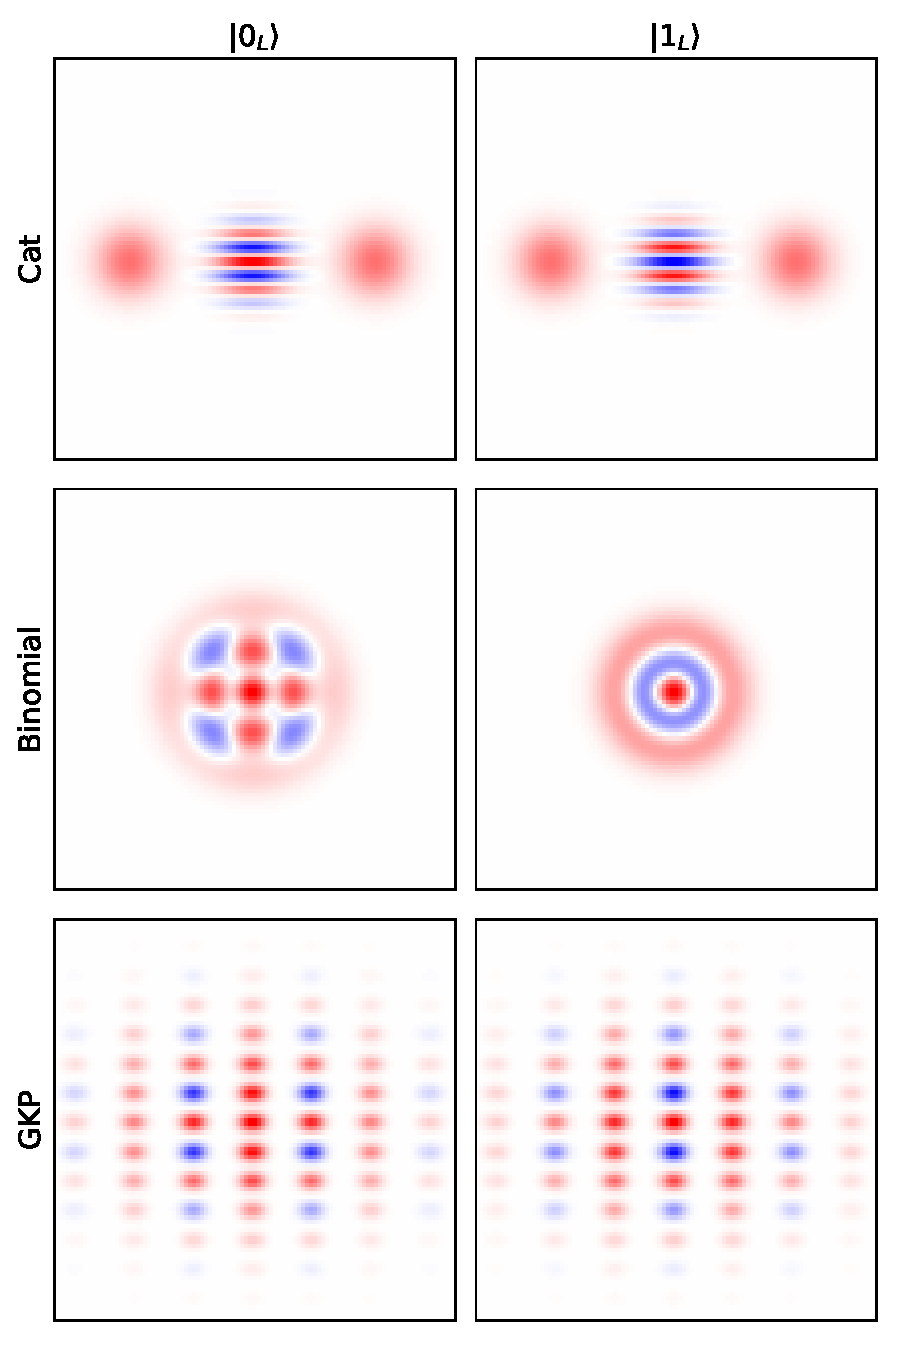
\includegraphics[width=0.8\columnwidth]{figures/cat_binom_gkp.pdf}
    \caption{Wigner functions for the logical qubit basis states in the cat, binomial, and GKP encodings.}
    \label{fig:cat_binom_gkp}
\end{figure}

Several bosonic encodings have been proposed.
For instance, binomial codes encode qubits as superpositions of Fock states, each of which is weighted by a binomial coefficient.
The lowest-order binomial code has logical basis states
\begin{align*}
    \ket{0_L} &= \left ( \ket{0} + \ket{4} \right ) / \sqrt{2}, \\
    \ket{1_L} &= \ket{2},
\end{align*}
and can protect against single-photon loss errors \cite{cai_2021,michael_2016}.
The Gottesman, Kitaev, and Preskill (GKP) code, on the other hand, defines the logical basis states as superpositions of squeezed states \cite{gottesman_2001}:
\begin{align*}
    \ket{0_L} &\propto \sum_{s=-\infty}^{\infty} \ket{q = 2 s \sqrt{\pi}}, \\
    \ket{1_L} &\propto \sum_{s=-\infty}^{\infty} \ket{q = (2 s + 1) \sqrt{\pi}}.
\end{align*}
The GKP code can protect against a variety of errors, but experimental implementation is difficult, and has only been demonstrated recently \cite{campagne_ibarcq_2020}.
See Cai et al. and Ma et al. \cite{cai_2021, ma_2021} for a review of recent progress in the area of bosonic error correction codes.
Figure \ref{fig:cat_binom_gkp} shows the Wigner functions for these two encodings, as well as the cat code we consider for the remainder of this paper.

Perhaps the simplest bosonic code is the so-called cat code, which encodes logical qubits as superpositions of coherent states of an oscillator opposite to each other in phase, i.e. Schr\"odinger cat states \cite{cai_2021,mirrahimi_2014,puri_2017,ofek_2016,grimm_2020,ma_2021}.
These states are given by
\[
    \ket{\mathcal{C}_\alpha^\pm} = \mathcal{N}_\alpha^\pm \left ( \ket{\alpha} \pm \ket{-\alpha} \right )
\]
where the normalization is
\[
    \mathcal{N}_\alpha^\pm = \frac {1} {\sqrt{ 2 \left ( 1 \pm e^{-2\bar{n}} \right ) }}
\]
for average photon number $\bar{n} = |\alpha|^2$.
In its simplest form the logical basis states in this encoding are
\begin{align*}
    \ket{0_L} &= \ket{\mathcal{C}_\alpha^+}, \\
    \ket{1_L} &= \ket{\mathcal{C}_\alpha^-}.
\end{align*}
Note that these states have opposite photon number parity: $\ket{\mathcal{C}_\alpha^+}$ only includes Fock states of even photon number parity, while those for $\ket{\mathcal{C}_\alpha^-}$ are only odd.

The separation in phase space of these opposite-phase coherent states ensures that the quantum information is protected from small, local displacements in phase \cite{mirrahimi_2014,grimm_2020}.
Note in particular the effect of the photon annihilation operator $\hat{a}$ on the cat states:
\[
    \hat{a} \ket{\mathcal{C}_\alpha^\pm} = \ket{\mathcal{C}_\alpha^\mp};
\]
that is, the loss of a photon from the resonator induces a bit flip error, which might be detected through continuous measurements of photon number parity.
Such an error detection is not possible in this simple realization of a cat qubit, but it has been implemented for more complex variations \cite{ofek_2016}.
Despite the lack of a means of detecting and correcting errors, this encoding is nonetheless a useful resource for quantum computation.
It has been shown that the noise in this encoding is ``biased'': phase flip errors are suppressed exponentially in $\bar{n}$, while the bit flip rate only increases linearly in $\bar{n}$ \cite{puri_2017,puri_2019}.
When the noise is biased in this manner, additional layers of QEC can focus on the dominant noise channel, i.e. bit flips.
Quantum logic gates that preserve this noise bias have been proposed, furthering the potential usefulness of this scheme \cite{puri_2020}.

The remainder of this paper is organized as follows: in Section \ref{sec:init} we discuss the initialization and stabilization of a cat qubit using a Kerr-nonlinear resonator and a two-photon squeezing drive.
In Section \ref{sec:gates} we discuss the implementation of single-qubit gates to drive rotations about the $X$ and $Z$ axes of the Bloch sphere.
In section \ref{sec:two_qubit} we extend the previous discussion of the operation of a single qubit to the case of two capacitively coupled Kerr-cat qubits.
For each aspect of the operation of these qubits we present numerical simulations using experimentally realistic parameters.
